\section{Experiments}\label{sec:experiments}

\begin{table}[t]
    \centering
    \begin{tabular}{c c}
        \begin{minipage}[b]{0.5\linewidth}
            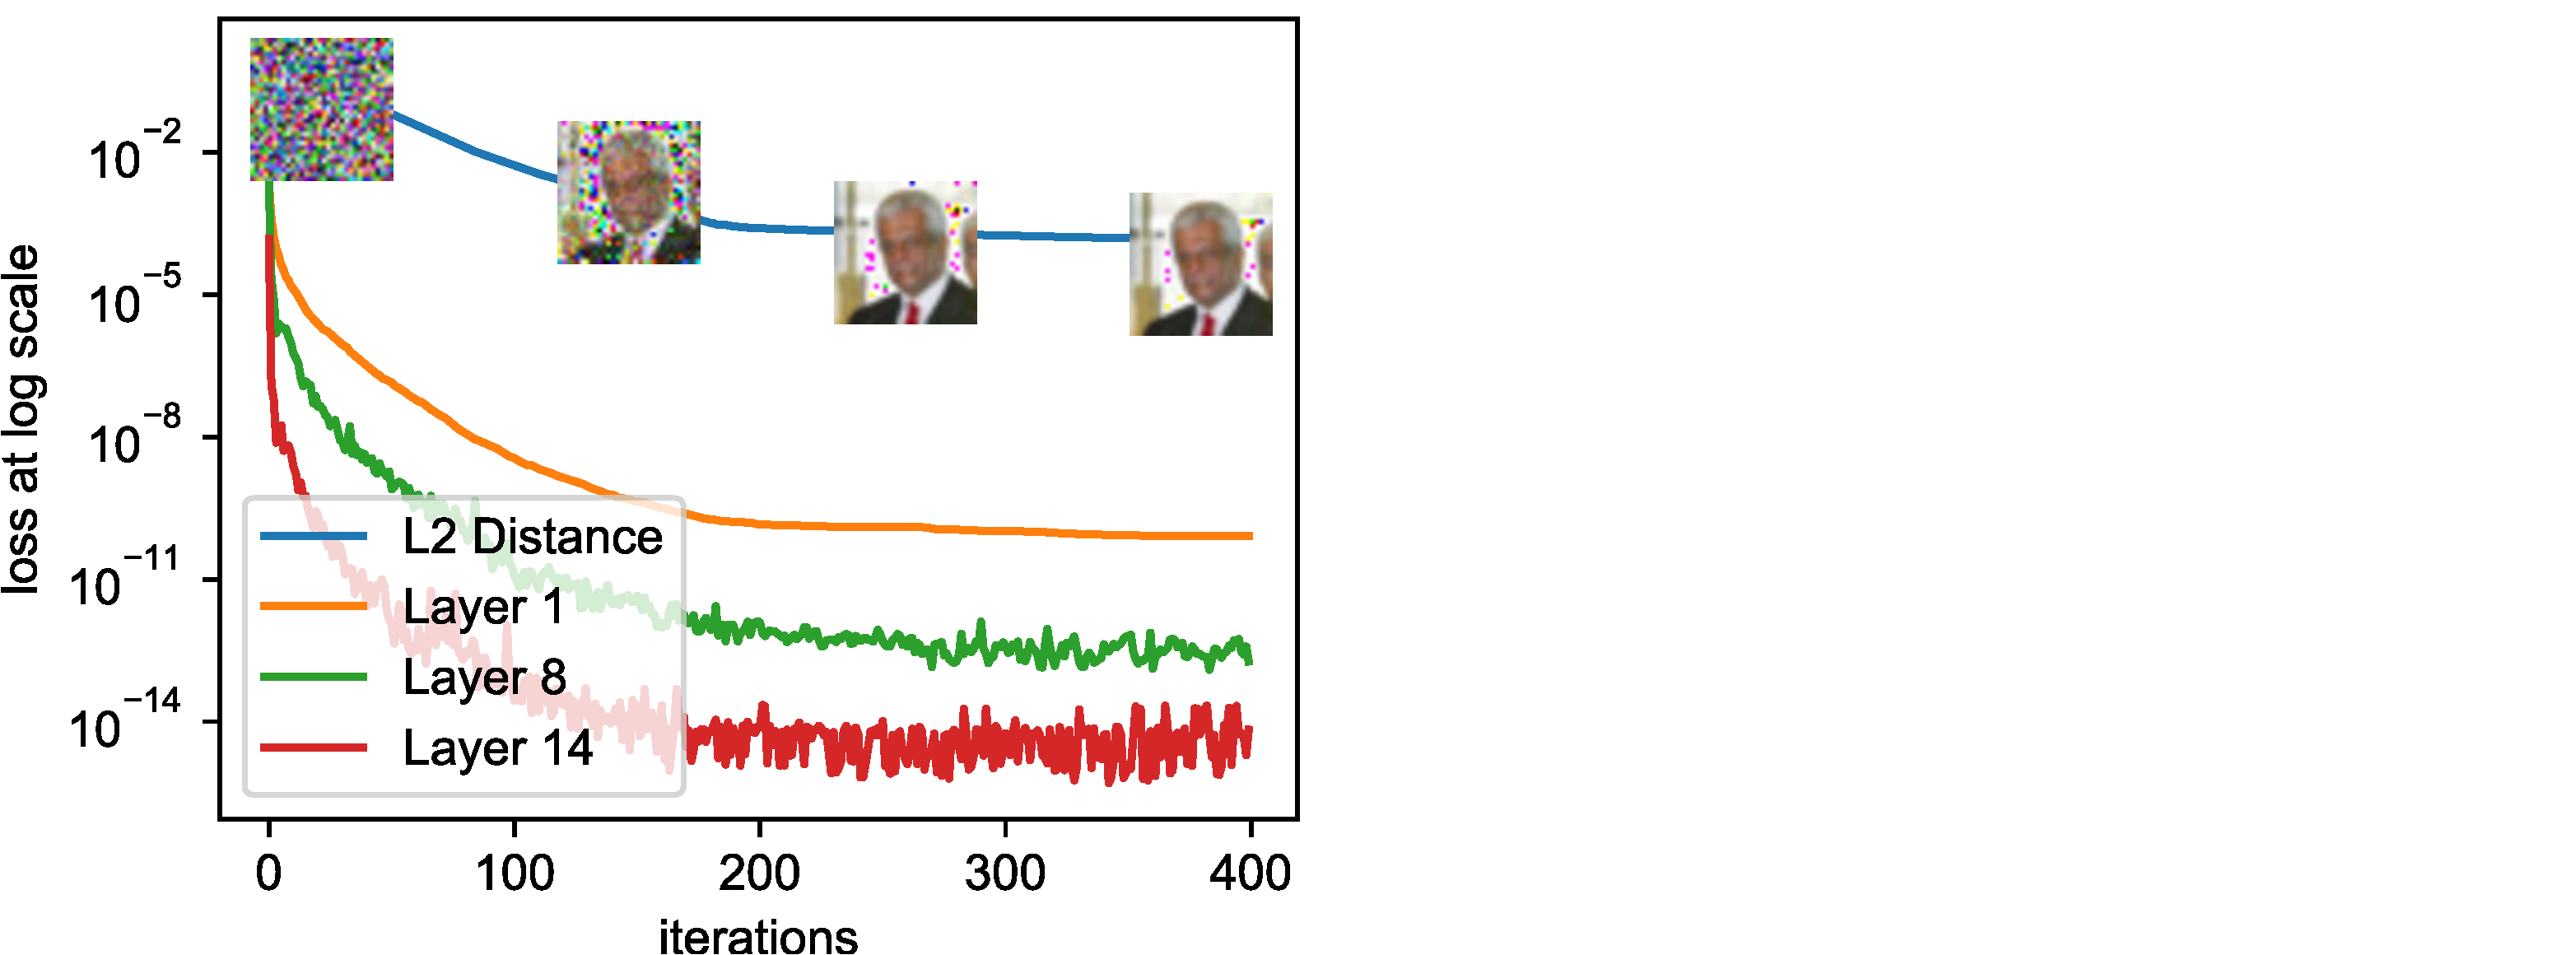
\includegraphics[width=\linewidth]{figures/fig3-crop.pdf}
            \captionof{figure}{Layer-$i$ means MSE between real and dummy gradients of $i^{th}$ layer.
            When the gradients' distance gets smaller, the MSE between leaked image and the original image also gets smaller.
            }
            \label{fig:vision_fig3}
        \end{minipage}
        &  
        \begin{minipage}[b]{0.45\linewidth}
        % \vspace{-20pt}
            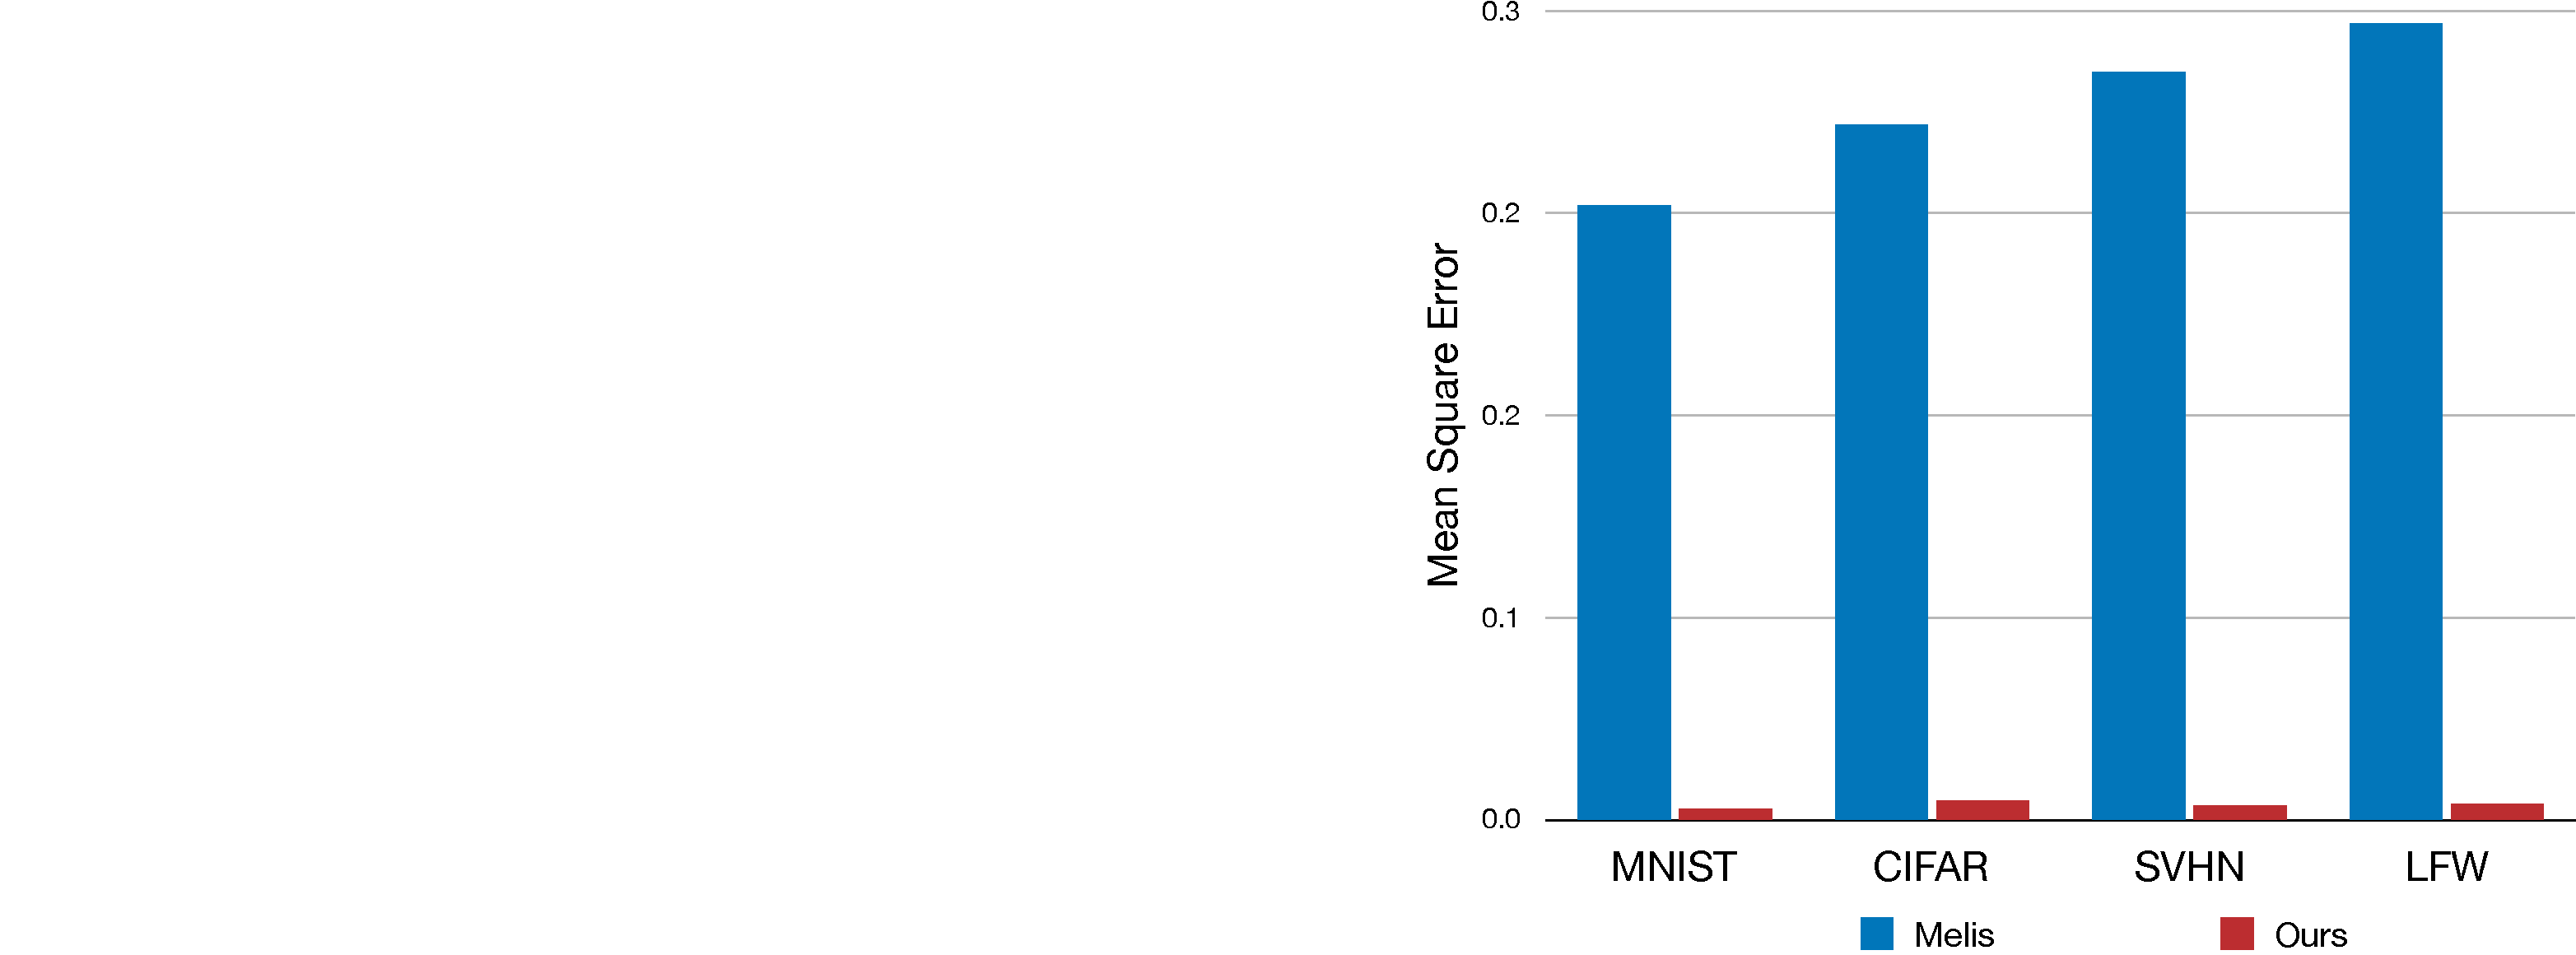
\includegraphics[width=\linewidth]{figures/fig4_barchart-crop.pdf}
            \captionof{figure}{Compassion of the MSE of images leaked by different algorithms and the ground truth. Our method consistently outperforms previous approach by a large margin.
            }
            \label{fig:vision_fig_bar}
        \end{minipage} 
    \end{tabular}
    \vspace{-10pt}
\end{table}


% We demonstrate the risks of deep leakage by two popular tasks -- image classification and natural language processing. It is worth noting that, though we only tested on two models, DLG can be extended to more machine learning models since the attack only requires the model to be differentiable. 

%%%%%%%%%%%%%%%%%%%%% IN SHORT: Setup 
\myparagraph{Setup.}
Implementing algorithm.~\ref{algorithm:deep_leakage} requires to calculate the high order gradients and we choose PyTorch~\cite{paszke2017pytorch} as our experiment platform. 
We use L-BFGS~\cite{liu1989lbfgs} with learning rate 1, history size 100 and max iterations 20 and optimize for 1200 iterations and 100 iterations for image and text task respectively. We aim to match gradients from all trainable parameters. Notably,
DLG has no requirements on model's convergence status, in another word, \textit{the attack can happen anytime during the training}. To be more general, all our experiments are using \textit{randomly initialized weights}. More task-specific details can be found in following sub-sections. 
% To make our experiments more reproducible, we attach our implementation in the appendix, with full details of the model architecture and parameter settings. (Colab codes will come soon.)

\subsection{Deep Leakage on Image Classification}
\label{sec:experiments_vision}

Given an image containing objects, images classification aims to determine the class of the item. We experiment our algorithm on modern CNN architectures ResNet-56~\cite{he2016deep} and pictures from MNIST~\cite{lecun1998mnist}, CIFAR-100~\cite{krizhevsky2009cifar}, SVHN~\cite{netzer2011svhn} and LFW~\cite{LFWTech}. Two changes we have made to the models are replacing activation ReLU to Sigmoid and removing strides, as our algorithm requires the model to be twice-differentiable. For image labels, instead of directly optimizing the discrete categorical values, we random initialize a vector with shape $N \times C$ where $N$ is the batch size and $C$ is the number of classes, and then take its softmax output as the one-hot label for optimization.

The leaking process is visualized in Fig.~\ref{fig:experiment_vision}. We start with random Gaussian noise (first column) and try to match the gradients produced by the dummy data and real ones. As shown in Fig~\ref{fig:vision_fig3}, minimizing the distance between gradients also reduces the gap between data. We observe that monochrome images with a clean background (MNIST) are easiest to recover, while complex images like face take more iterations to recover (Fig.~\ref{fig:experiment_vision}). When the optimization finishes, the recover results are almost identical to ground truth images, despite few negligible artifact pixels.

We visually compare the results from other method~\cite{Melis2018unintended} and ours in Fig.~\ref{fig:experiment_vision}. 
The previous method uses GAN models when the class label is given and only works well on MNIST. The result on SVHN, though is still visually recognizable as digit ``9'', this is no longer the original training image. The cases are even worse on LFW and collapse on CIFAR. We also make a numerical comparison by performing leaking and measuring the MSE on all dataset images in Fig.~\ref{fig:vision_fig_bar}. Images are normalized to the range $[0, 1]$ and our algorithm appears much better results (ours $< 0.03$ v.s. previous $> 0.2$) on all four datasets.


\subsection{Deep Leakage on Masked Language Model} \label{sec:experiments_nlp}
\begin{table}[t]
    \centering
    \small
    \begin{tabular}{p{0.10\linewidth}|p{0.25\linewidth}|p{0.25\linewidth}|p{0.25\linewidth}}
         & Example 1 & Example 2 & Example 3\\ \hline
        Initial Sentence
        & tilting fill given **less word **itude fine **nton overheard living vegas **vac **vation *f forte **dis cerambycidae ellison **don yards marne **kali
        & toni **enting asbestos cutler km nail **oof **dation **ori righteous **xie lucan **hot **ery at **tle ordered pa **eit smashing proto
        & [MASK] **ry toppled **wled major relief dive displaced **lice [CLS] us apps \_ **face **bet
    \\ \hline
        Iters = 10 
        & tilting fill given **less full solicitor other ligue shrill living vegas rider treatment carry played sculptures lifelong ellison net yards marne **kali
        & toni **enting asbestos cutter km nail undefeated **dation hole righteous **xie lucan **hot **ery at **tle ordered pa **eit smashing proto
        & [MASK] **ry toppled identified major relief gin dive displaced **lice doll us apps \_ **face space
    \\ \hline
        Iters = 20 
        & registration , volunteer applications , at student travel application open the ; week of played ; child care will be glare .
        & we welcome proposals for tutor **ials on either core machine denver softly or topics of emerging importance for machine learning .
        & one **ry toppled hold major ritual ' dive annual conference days 1924 apps novelist dude space
    \\ \hline
        Iters = 30 
        & registration , volunteer applications , and student travel application open the first week of september . child care will be available .
        & we welcome proposals for tutor **ials on either core machine learning topics or topics of emerging importance for machine learning .
        & we invite submissions for the thirty - third annual conference on neural information processing systems .
    \\ \hline
        Original Text 
        & Registration, volunteer applications, and student travel application open the first week of September. Child care will be available.
        & We welcome proposals for tutorials on either core machine learning topics or topics of emerging importance for machine learning.
        & We invite submissions for the Thirty-Third Annual Conference on Neural Information Processing Systems.
    \end{tabular}
    \caption{The progress of deep leakage on language tasks. }
    \vspace{-5pt}
    \label{tab:experiment_nlp}
\end{table}


For language task, we verify our algorithm on Masked Language Model (MLM) task. In each sequence, 15\% of the words are replaced with a [MASK] token and MLM model attempts to predict the original value of the masked words from a given context. We choose BERT~\cite{devlin2018bert} as our backbone and adapt hyperparameters from the official implementation~\footnote{\url{https://github.com/google-research/bert}}.

Different from vision tasks where RGB inputs are continuous values, language models need to preprocess discrete words into embeddings. We apply DLG on embedding space and minimize the gradients distance between dummy embeddings and real ones. After optimization finishes, we derive original words by finding the closest entry in the embedding matrix reversely. 

In Tab.~\ref{tab:experiment_nlp}, we exhibit the leaking history on three sentences selected from NeurIPS conference page. Similar to the vision task, we start with randomly initialized embedding: the reverse query results at iteration 0 is meaningless. During the optimization, the gradients produced by dummy embedding gradually match the original ones and so the embeddings. In later iterations, part of sequence gradually appears. In example 3, at iteration 20, `annual conference' appeared and at iteration 30 and the leaked sentence is already close to the original one. When DLG finishes, though there are few mismatches caused by the ambiguity in tokenizing, the main content is already fully leaked.
